% Options for packages loaded elsewhere
\PassOptionsToPackage{unicode}{hyperref}
\PassOptionsToPackage{hyphens}{url}
%
\documentclass[
]{book}
\usepackage{amsmath,amssymb}
\usepackage{lmodern}
\usepackage{iftex}
\ifPDFTeX
  \usepackage[T1]{fontenc}
  \usepackage[utf8]{inputenc}
  \usepackage{textcomp} % provide euro and other symbols
\else % if luatex or xetex
  \usepackage{unicode-math}
  \defaultfontfeatures{Scale=MatchLowercase}
  \defaultfontfeatures[\rmfamily]{Ligatures=TeX,Scale=1}
\fi
% Use upquote if available, for straight quotes in verbatim environments
\IfFileExists{upquote.sty}{\usepackage{upquote}}{}
\IfFileExists{microtype.sty}{% use microtype if available
  \usepackage[]{microtype}
  \UseMicrotypeSet[protrusion]{basicmath} % disable protrusion for tt fonts
}{}
\makeatletter
\@ifundefined{KOMAClassName}{% if non-KOMA class
  \IfFileExists{parskip.sty}{%
    \usepackage{parskip}
  }{% else
    \setlength{\parindent}{0pt}
    \setlength{\parskip}{6pt plus 2pt minus 1pt}}
}{% if KOMA class
  \KOMAoptions{parskip=half}}
\makeatother
\usepackage{xcolor}
\IfFileExists{xurl.sty}{\usepackage{xurl}}{} % add URL line breaks if available
\IfFileExists{bookmark.sty}{\usepackage{bookmark}}{\usepackage{hyperref}}
\hypersetup{
  pdftitle={FH Cluster Guide},
  hidelinks,
  pdfcreator={LaTeX via pandoc}}
\urlstyle{same} % disable monospaced font for URLs
\usepackage{longtable,booktabs,array}
\usepackage{calc} % for calculating minipage widths
% Correct order of tables after \paragraph or \subparagraph
\usepackage{etoolbox}
\makeatletter
\patchcmd\longtable{\par}{\if@noskipsec\mbox{}\fi\par}{}{}
\makeatother
% Allow footnotes in longtable head/foot
\IfFileExists{footnotehyper.sty}{\usepackage{footnotehyper}}{\usepackage{footnote}}
\makesavenoteenv{longtable}
\usepackage{graphicx}
\makeatletter
\def\maxwidth{\ifdim\Gin@nat@width>\linewidth\linewidth\else\Gin@nat@width\fi}
\def\maxheight{\ifdim\Gin@nat@height>\textheight\textheight\else\Gin@nat@height\fi}
\makeatother
% Scale images if necessary, so that they will not overflow the page
% margins by default, and it is still possible to overwrite the defaults
% using explicit options in \includegraphics[width, height, ...]{}
\setkeys{Gin}{width=\maxwidth,height=\maxheight,keepaspectratio}
% Set default figure placement to htbp
\makeatletter
\def\fps@figure{htbp}
\makeatother
\setlength{\emergencystretch}{3em} % prevent overfull lines
\providecommand{\tightlist}{%
  \setlength{\itemsep}{0pt}\setlength{\parskip}{0pt}}
\setcounter{secnumdepth}{5}
\ifLuaTeX
  \usepackage{selnolig}  % disable illegal ligatures
\fi

\title{FH Cluster Guide}
\author{}
\date{\vspace{-2.5em}September 23, 2022}

\begin{document}
\maketitle

{
\setcounter{tocdepth}{1}
\tableofcontents
}
\hypertarget{about-this-course}{%
\chapter*{About this Course}\label{about-this-course}}
\addcontentsline{toc}{chapter}{About this Course}

Our goal is to get you running on the Fred Hutch cluster quickly and efficiently with this quick-start guide. As a wise Drivers' Ed instructor once said, \textbf{you need to go slow to go fast}!

In this short course, you'll invest a bit of time now to save you time and frustration down the road. Follow along at \textbf{any time on your own schedule}. We hope that the following modules will help you take advantage of the powerful resources the Fred Hutch has to offer!

\hypertarget{part-cluster-101}{%
\part*{Cluster 101}\label{part-cluster-101}}
\addcontentsline{toc}{part}{Cluster 101}

\hypertarget{what-is-a-cluster}{%
\chapter{What is a Cluster?}\label{what-is-a-cluster}}

A computing cluster is a set of many computers networked together. Because there are many computers working together, the network is able to handle computationally expensive tasks, like genome assemblies or advanced algorithms. Imagine you're building a house. It would take a long time by yourself! It's much better to have many builders working together.

Now that we have a team of workers, the next challenge is task management. A home construction team will need a manager to help delegate tasks. Similarly, the computing cluster uses management software to prioritize tasks, delegate workers (resources), and check on progress. The Fred Hutch cluster uses a common management and scheduling tool called \href{https://slurm.schedmd.com/overview.html}{Slurm}.

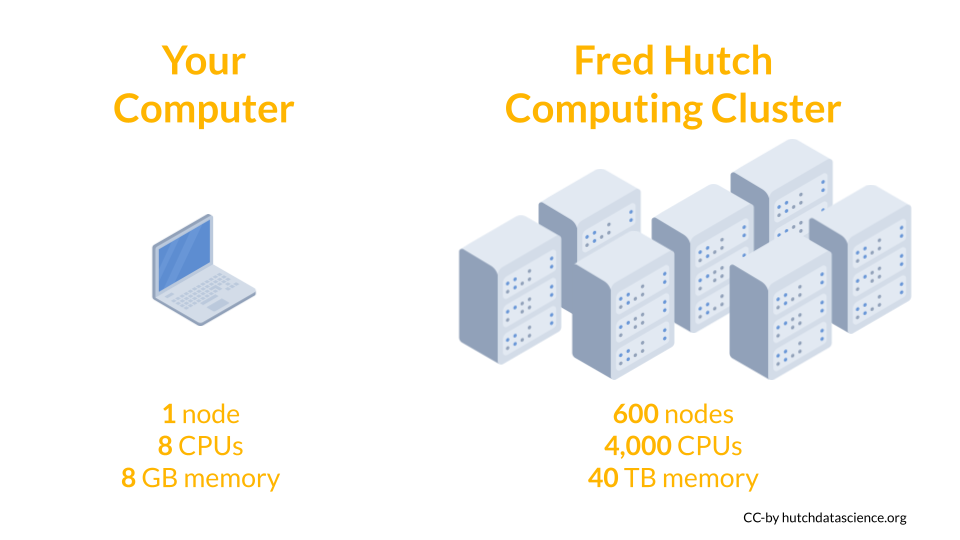
\includegraphics[width=1\linewidth]{resources/images/01-101_files/figure-latex//1BQxrVYdKZTbpCaF-i_q9w7s9x034lEXpQZDU-Sl09cs_g149d37dd4a1_0_18}

How is the cluster different from a laptop or desktop? First, you might use an operating system like Windows or MacOS. The Fred Hutch server is a Linux system. Second, because many people use the cluster for many tasks, there isn't a central screen and keyboard. You access the cluster remotely from your computer! We will talk more about how to connect to the cluster in a \protect\hyperlink{terminal}{following chapter}.

\textbf{Computing cluster}

A set of computers networked together to perform large tasks.

\hypertarget{account-setup}{%
\chapter{Account Setup}\label{account-setup}}

You will need an account to log in to the cluster. This ensures that data stays protected.

\hypertarget{check-your-hutchnet-id}{%
\section{Check your HutchNet ID}\label{check-your-hutchnet-id}}

Your \href{https://centernet.fredhutch.org/cn/u/center-it/help-desk.html}{HutchNet ID} is the standard login you receive when you start working at the Hutch or are an official affiliate. You can use it to login to most resources at the Center (Desktop Computer, Employee Self Service, VPN, Webmail) and our Scientific Computing systems.

For example:

\begin{itemize}
\tightlist
\item
  my email is \texttt{jsmith3@fredhutch.org}.\\
\item
  my HutchNet ID is \texttt{jsmith3}.
\end{itemize}

If one of your collaborators requires access to the Fred Hutch network you can submit a \href{https://centernet.fredhutch.org/cn/f/hr/lcex/non-employee-action-form.html}{non-employee action form}. Non-employee is a generic administrative term for affiliates, students, contractors, etc.

\hypertarget{contacting-the-scicomp-team}{%
\section{Contacting the SciComp Team}\label{contacting-the-scicomp-team}}

To use Scientific Computing clusters at Hutch, your HutchNet ID must be associated with a PI account.

The Scientific Computing Team (SciComp) tries to set some users up ahead of time. However, not everyone is set up automatically. Please fill out \href{https://forms.gle/5ct8mQCeBD7LUt6S7}{this Account Setup Form} and we will ensure you are set up correctly!

Errors similar to ``Invalid account or account/partition'' typically indicate that the account hasn't been set up by SciComp. This is a quick fix if you use the form above.

Now, let's set up our Terminal!

\hypertarget{terminal}{%
\chapter{Terminal Setup}\label{terminal}}

The next step is getting familiar with your Terminal. This is your portal to the cluster.

\hypertarget{what-is-a-terminal}{%
\section{What is a terminal?}\label{what-is-a-terminal}}

The Terminal is a \href{https://www.codecademy.com/article/command-line-interface}{command line interface}. In other words, the Terminal is a software application that allows you to issue commands directly to your laptop or desktop computer. The Terminal is very useful because it allows you to run commands that don't have a graphical user interface (GUI). It can also connect you to computer networks, such as the Fred Hutch cluster! The Terminal setup is different depending on your operating system. Jump to the \protect\hyperlink{windows}{Windows}, \protect\hyperlink{mac}{MacOS}, or \protect\hyperlink{linux}{Linux} sections below.

``Terminal'' used to be synonymous with ``computer''. With the creation of operating systems like Windows and MacOS, computers became much easier to use and exploded in popularity! Your colleagues are almost always referring to the command line application when they say ``Terminal''.

\hypertarget{windows}{%
\section{Windows Setup}\label{windows}}

Click to view steps

You will need to install a Terminal application called PuTTY to connect to the Fred Hutch Cluster.

\begin{enumerate}
\def\labelenumi{\arabic{enumi}.}
\item
  You should then see PuTTY available in the Software Center. Click ``Install'' and go through the Setup Wizard.

  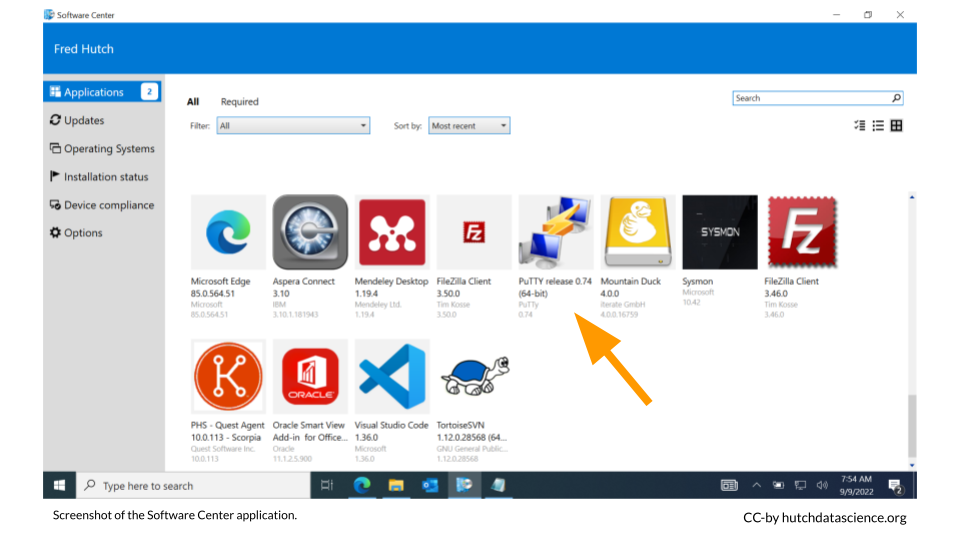
\includegraphics[width=1\linewidth]{resources/images/01-101_files/figure-latex//1BQxrVYdKZTbpCaF-i_q9w7s9x034lEXpQZDU-Sl09cs_g15643d101eb_4_15}

  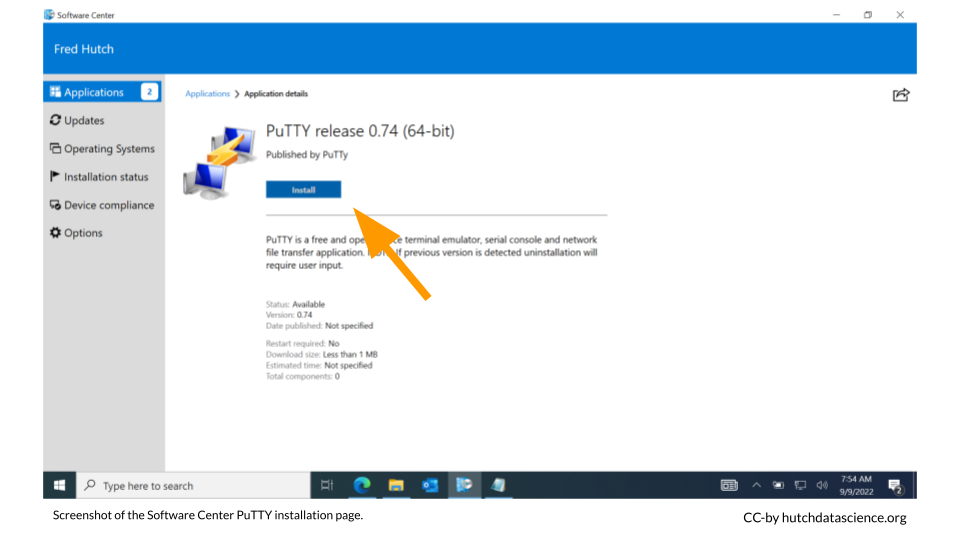
\includegraphics[width=1\linewidth]{resources/images/01-101_files/figure-latex//1BQxrVYdKZTbpCaF-i_q9w7s9x034lEXpQZDU-Sl09cs_g15643d101eb_4_20}

  You can also \href{faq.html\#manual-putty}{install PuTTY manually} if you don't see it in the Software Center.
\item
  PuTTY should now be available in your applications. Click on PuTTY to open.

  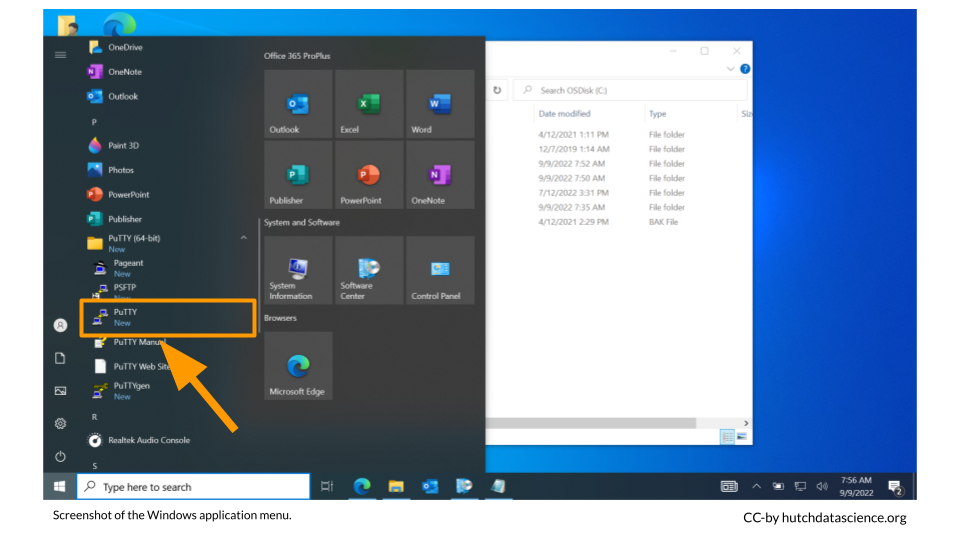
\includegraphics[width=1\linewidth]{resources/images/01-101_files/figure-latex//1BQxrVYdKZTbpCaF-i_q9w7s9x034lEXpQZDU-Sl09cs_g15643d101eb_4_28}
\item
  You should now see the PuTTY Configuration menu.

  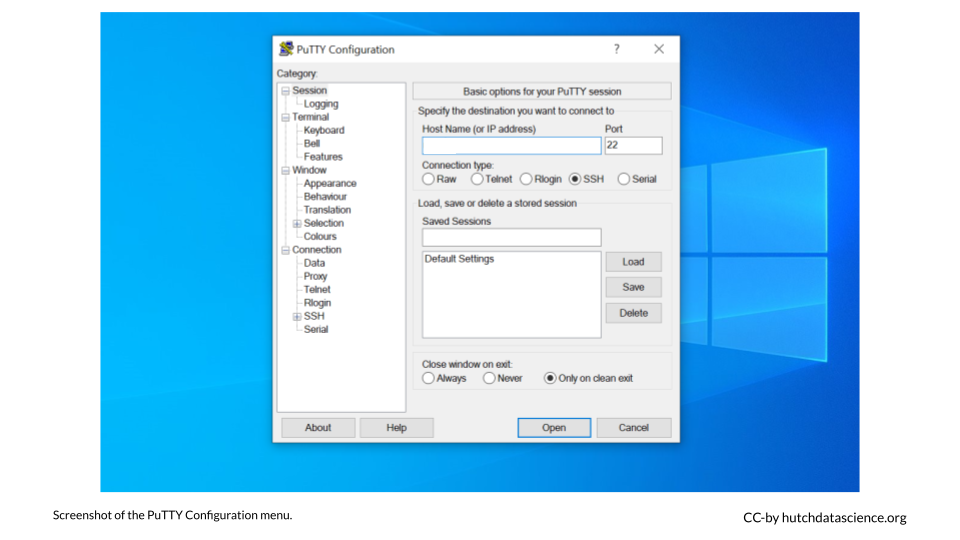
\includegraphics[width=1\linewidth]{resources/images/01-101_files/figure-latex//1BQxrVYdKZTbpCaF-i_q9w7s9x034lEXpQZDU-Sl09cs_g15643d101eb_4_35}
\end{enumerate}

\hypertarget{mac}{%
\section{Mac Setup}\label{mac}}

Click to view steps

Mac machines come with a Terminal installed.

\begin{enumerate}
\def\labelenumi{\arabic{enumi}.}
\item
  Go to Finder \textgreater{} Applications \textgreater{} Utilities \textgreater{} Terminal and double-click.

  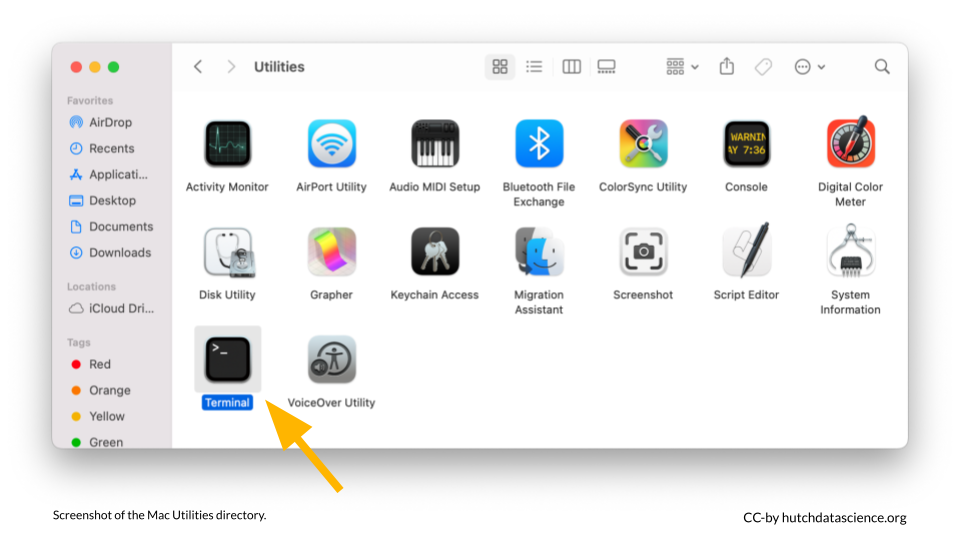
\includegraphics[width=1\linewidth]{resources/images/01-101_files/figure-latex//1BQxrVYdKZTbpCaF-i_q9w7s9x034lEXpQZDU-Sl09cs_g149d37dd4a1_0_9}
\item
  Your Terminal should look like this:

  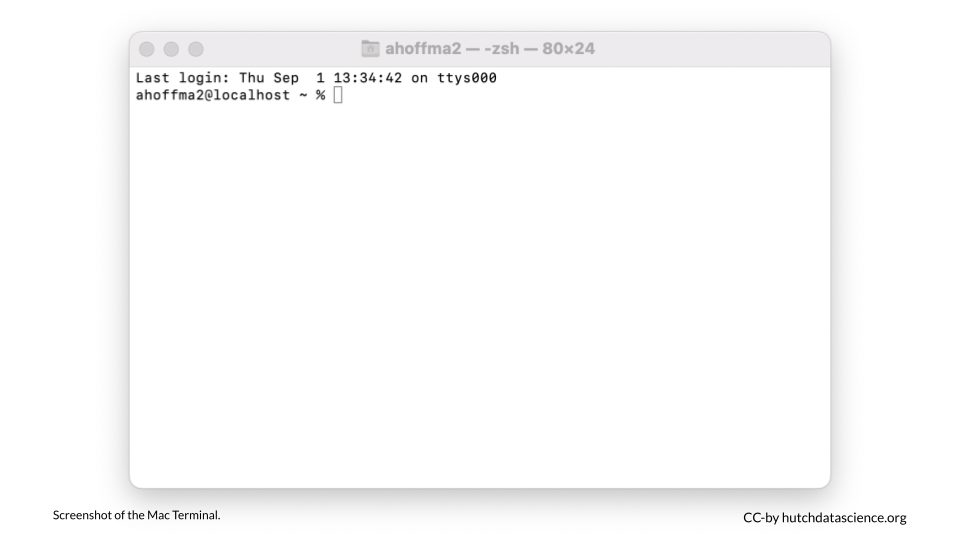
\includegraphics[width=1\linewidth]{resources/images/01-101_files/figure-latex//1BQxrVYdKZTbpCaF-i_q9w7s9x034lEXpQZDU-Sl09cs_g149d37dd4a1_0_2}
\end{enumerate}

\hypertarget{linux}{%
\section{Linux Setup}\label{linux}}

Click to view steps

The commonly used Linux distribution, Ubuntu, already comes with a Terminal installed.

\begin{enumerate}
\def\labelenumi{\arabic{enumi}.}
\tightlist
\item
  Press ctrl + alt + T. Your open Terminal window should look like this:
\end{enumerate}

{[}SCREENSHOT{]}

\begin{enumerate}
\def\labelenumi{\arabic{enumi}.}
\tightlist
\item
  Update the Terminal and prepare it for connecting to the cluster by running:
\end{enumerate}

\begin{verbatim}
sudo apt install openssh-server
\end{verbatim}

Enter your password and enter \texttt{Y} when prompted.

\hypertarget{logging-in}{%
\chapter{Logging In}\label{logging-in}}

Now that you have your Terminal application ready, you want to connect to the cluster. You will do this using a method called \href{https://www.ssh.com/academy/ssh/protocol}{SSH}, which stands for ``Secure SHell''.

\hypertarget{what-is-ssh}{%
\section{\texorpdfstring{What is \texttt{SSH}?}{What is SSH?}}\label{what-is-ssh}}

SSH is a secure way to remotely connect to another computer or network of computers. In other words, SSH helps us protect your data and the data on the Fred Hutch cluster through authentication.

\textbf{Hostname}

The hostname is the name, or label, assigned to a computer in a network. We are connecting to hostname \texttt{rhino.fhcrc.org} or \texttt{rhino} for short.

Before moving on, you will need to connect to the Fred Hutch wifi network, a networked ethernet jack, or the \href{https://centernet.fredhutch.org/cn/u/center-it/help-desk/vpn.html}{Fred Hutch VPN}. This is the first layer of security.

The next set of steps are specific to your operating system.

\hypertarget{windows-login}{%
\section{Windows Login}\label{windows-login}}

Click to view steps

\begin{enumerate}
\def\labelenumi{\arabic{enumi}.}
\item
  Go to the PuTTY Configuration menu. Under ``Host Name'' type \textbf{rhino} and click ``Open''.

  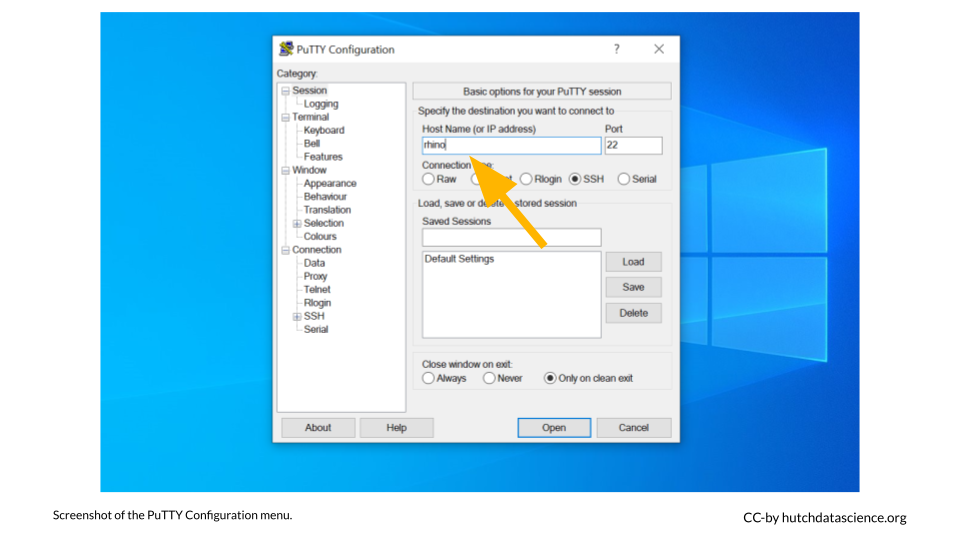
\includegraphics[width=1\linewidth]{resources/images/01-101_files/figure-latex//1BQxrVYdKZTbpCaF-i_q9w7s9x034lEXpQZDU-Sl09cs_g15643d101eb_4_41}
\item
  You will be prompted to login. Type in your HutchNetID (e.g., \texttt{jsmith3}).

  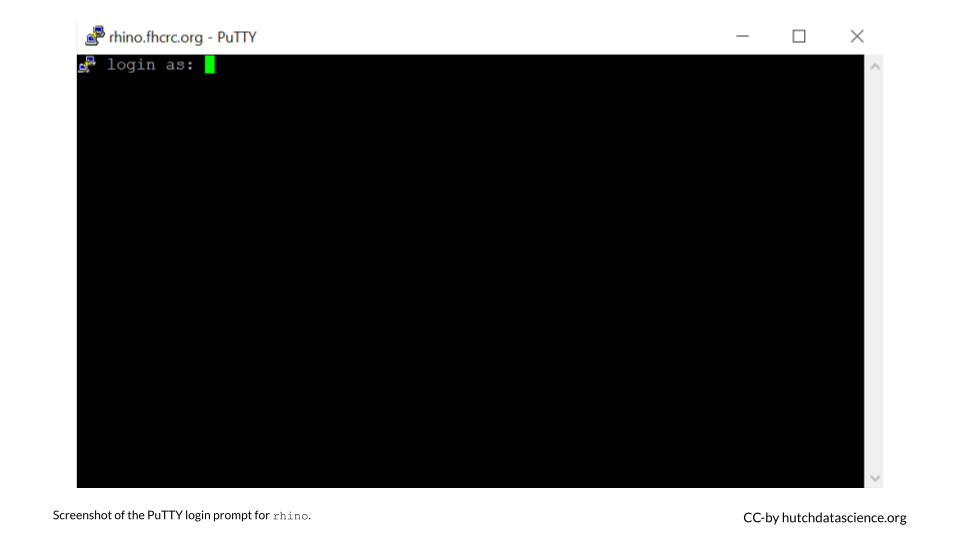
\includegraphics[width=1\linewidth]{resources/images/01-101_files/figure-latex//1BQxrVYdKZTbpCaF-i_q9w7s9x034lEXpQZDU-Sl09cs_g15643d101eb_4_48}
\item
  Enter your password. No\texttt{*} or symbols will show up, so type it in carefully!
\item
  You are now logged in! There should be a login message, with your name at the bottom.

  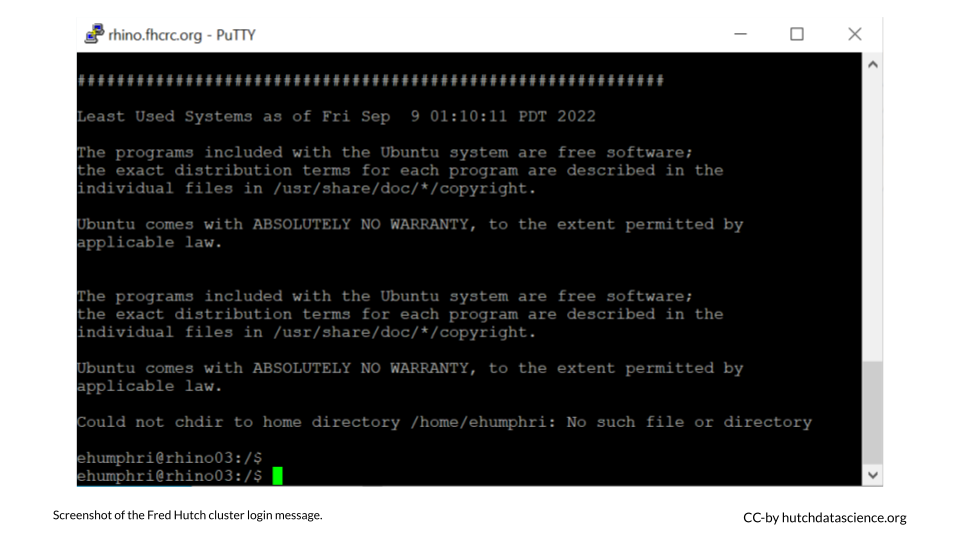
\includegraphics[width=1\linewidth]{resources/images/01-101_files/figure-latex//1BQxrVYdKZTbpCaF-i_q9w7s9x034lEXpQZDU-Sl09cs_g15643d101eb_4_60}
\end{enumerate}

Congratulations! You are now logged in to the Fred Hutch cluster!

\hypertarget{mac-login}{%
\section{Mac Login}\label{mac-login}}

Click to view steps

\begin{enumerate}
\def\labelenumi{\arabic{enumi}.}
\item
  Type the following commands, substituting in your HutchNet ID:

\begin{verbatim}
ssh -Y HutchID@rhino
\end{verbatim}
\item
  You will see a message that looks like \texttt{The\ authenticity\ of\ host\ \textquotesingle{}rhino\ (XXX.XXX.XX.XX)\textquotesingle{}\ can\textquotesingle{}t\ be\ established.} Type in \texttt{yes} and hit enter.
\item
  Enter your password. No\texttt{*} or symbols will show up, so type it in carefully!
\item
  You are now logged in! There should be a login message, with your name at the bottom.

  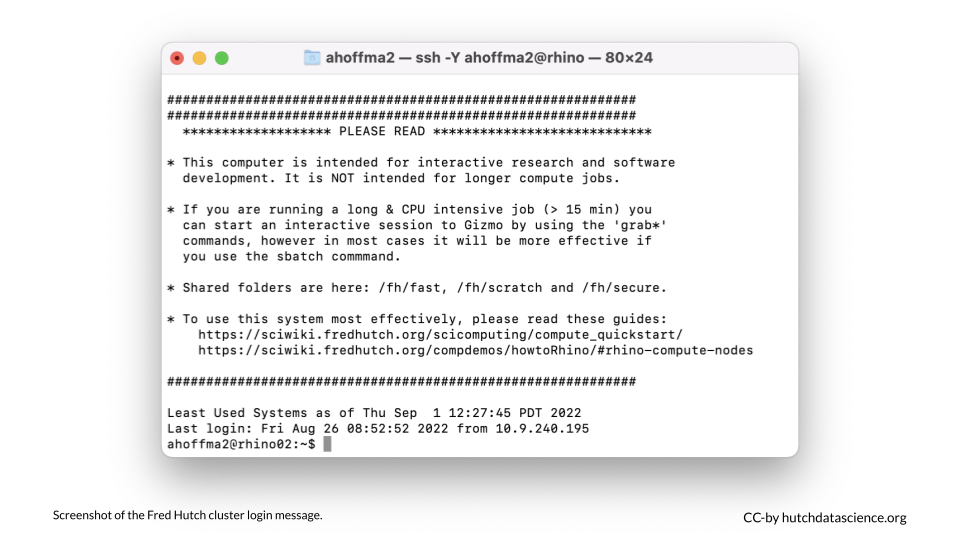
\includegraphics[width=1\linewidth]{resources/images/01-101_files/figure-latex//1BQxrVYdKZTbpCaF-i_q9w7s9x034lEXpQZDU-Sl09cs_g149d37dd4a1_0_43}
\end{enumerate}

Congratulations! You are now logged in to the Fred Hutch cluster!

\hypertarget{linux-login}{%
\section{Linux Login}\label{linux-login}}

Click to view steps

Congratulations! You are now logged in to the Fred Hutch cluster!

\hypertarget{submit-your-first-job}{%
\chapter{Submit Your First Job}\label{submit-your-first-job}}

The Fred Hutch cluster uses \href{https://slurm.schedmd.com/overview.html}{Slurm} to organize and prioritize jobs. Instead of running commands directly on rhino, you will submit a script (a snippet of directions) to tell Slurm what to do.

\hypertarget{download-the-script}{%
\section{Download the Script}\label{download-the-script}}

We can use the \texttt{wget} command to download a script from GitHub. This means we don't have to write the script from scratch. Copy and paste the following into the terminal, and hit return:

\begin{verbatim}
wget https://raw.githubusercontent.com/FredHutch/slurm-examples/master/introduction/1-hello-world/01.sh
\end{verbatim}

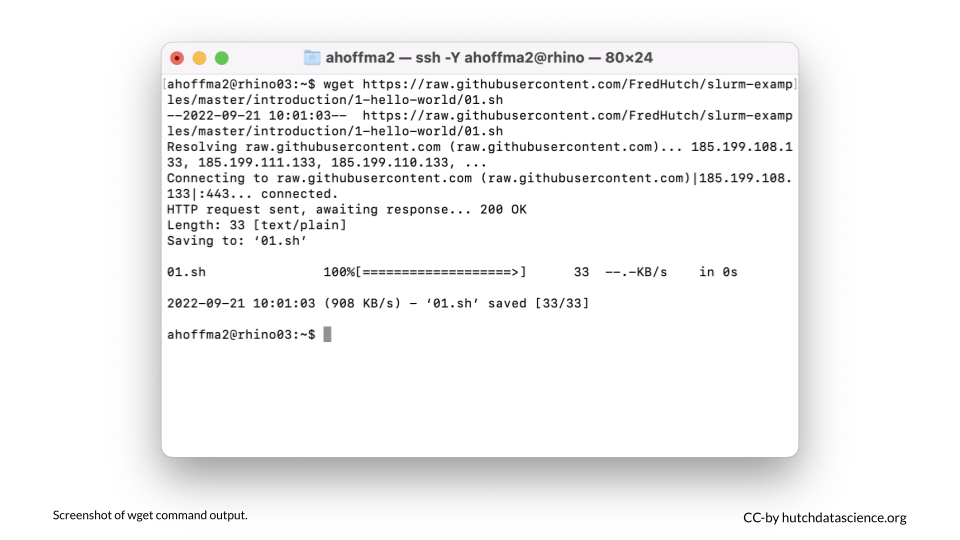
\includegraphics[width=1\linewidth]{resources/images/01-101_files/figure-latex//1BQxrVYdKZTbpCaF-i_q9w7s9x034lEXpQZDU-Sl09cs_g1579ffd7b01_0_0}

\hypertarget{confirm-the-download}{%
\section{Confirm the Download}\label{confirm-the-download}}

Let's confirm that we can see the file we just downloaded. We can use the \texttt{ls} (list files) command for this. Type \texttt{ls} and hit return. You should see the file \texttt{01.sh} in your home directory. The \texttt{.sh} ending means this is a script meant to run from the command line.

\begin{verbatim}
ls
\end{verbatim}

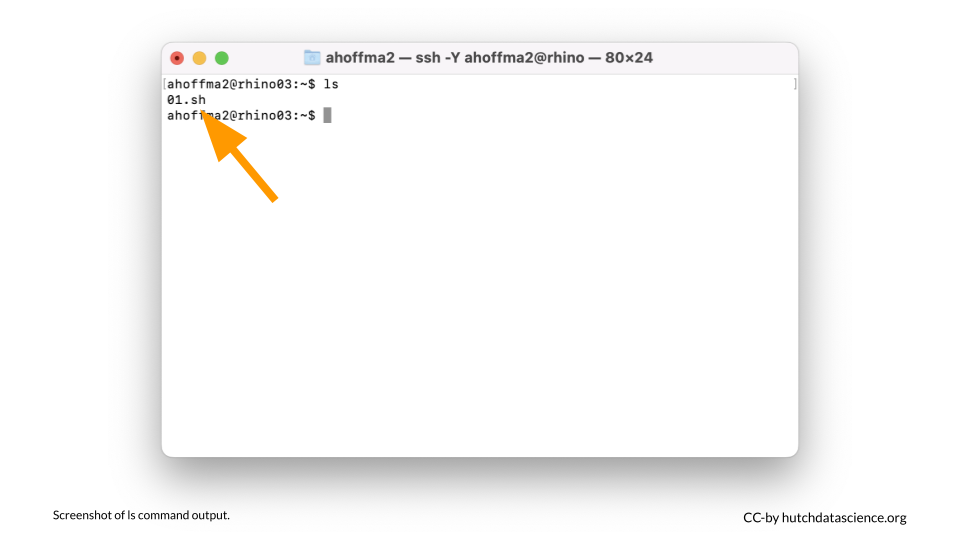
\includegraphics[width=1\linewidth]{resources/images/01-101_files/figure-latex//1BQxrVYdKZTbpCaF-i_q9w7s9x034lEXpQZDU-Sl09cs_g1579ffd7b01_0_6}

\hypertarget{inspect-the-script}{%
\section{Inspect the Script}\label{inspect-the-script}}

Let's next inspect the script. The \texttt{cat} command, followed by a file name, lists the entire contents of a specific file.

\begin{verbatim}
cat 01.sh
\end{verbatim}

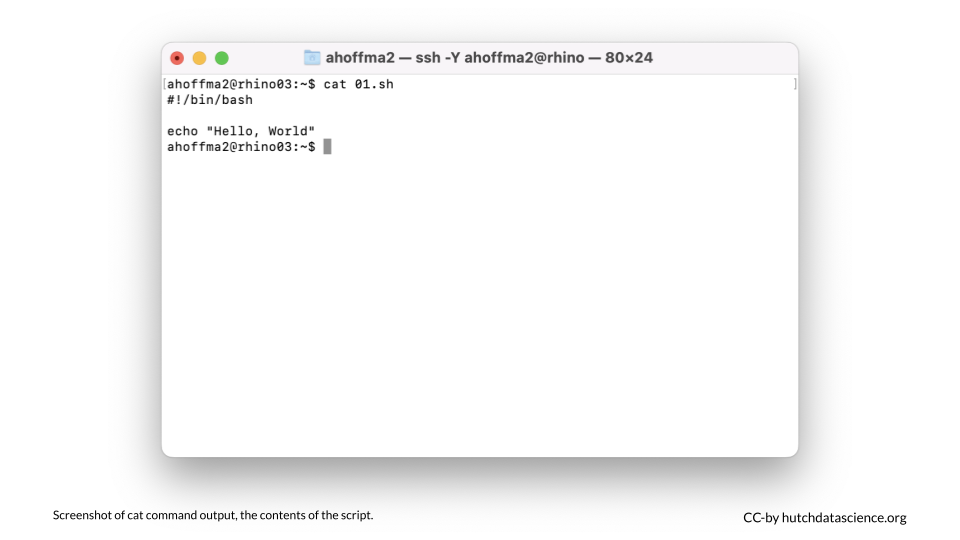
\includegraphics[width=1\linewidth]{resources/images/01-101_files/figure-latex//1BQxrVYdKZTbpCaF-i_q9w7s9x034lEXpQZDU-Sl09cs_g1579ffd7b01_12_2}

\begin{itemize}
\tightlist
\item
  The first line of the script, \texttt{\#!/bin/bash}, indicates that this is a command line or ``bash'' script.
\item
  The second line is empty, and the third line, \texttt{echo\ "Hello,\ World"} means that the computer will ``echo'', or print out, ``Hello, World''.
\end{itemize}

\hypertarget{submit-the-script}{%
\section{Submit the Script}\label{submit-the-script}}

We use the \texttt{sbatch} command to submit a script and start running a job on the cluster. Copy the following and hit return. You should see a message like ``\texttt{Submitted\ batch\ job\ 12345678}''. Your number will vary because this is a unique job identifier.

\begin{verbatim}
sbatch 01.sh
\end{verbatim}

\hypertarget{check-the-output}{%
\section{Check the Output}\label{check-the-output}}

Type \texttt{ls} again. You should now see a log file like \texttt{slurm-12345678.out} listed alongside your script \texttt{01.sh}. Let's use \texttt{cat} to inspect the output in the log file. We should see our message has been printed!

\begin{verbatim}
cat slurm-<your-number-here>.out
\end{verbatim}

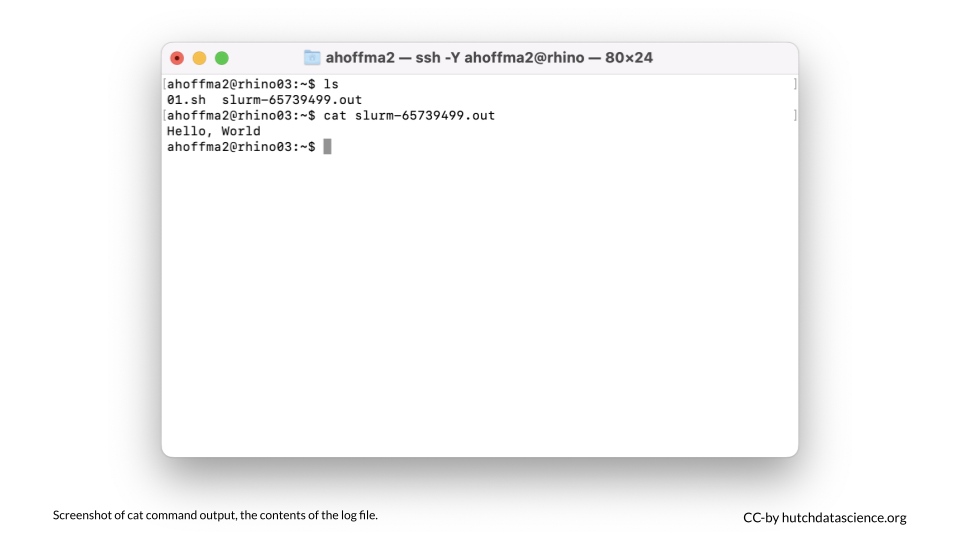
\includegraphics[width=1\linewidth]{resources/images/01-101_files/figure-latex//1BQxrVYdKZTbpCaF-i_q9w7s9x034lEXpQZDU-Sl09cs_g1579ffd7b01_12_22}

\texttt{ls}

This command lists the files in the current directory.

\texttt{cat} \emph{filename}

This command prints the contents of a specific file .

\texttt{sbatch} \emph{filename.sh}

This command submits a job to the cluster with instructions specified in .sh

\hypertarget{file-upload-and-download}{%
\chapter{File Upload and Download}\label{file-upload-and-download}}

Exchanging files with the cluster is very important. You can imagine scenarios where:

\begin{itemize}
\tightlist
\item
  You want to download log files or output files
\item
  You want to upload a custom \texttt{.sh} script file that you wrote on your laptop
\item
  You want to upload other files
\end{itemize}

In this course, upload and download of files is performed using \href{https://cyberduck.io/}{Cyberduck}. Cyberduck is a tool that lets us connect to the cluster securely, browse files, and transfer files securely.

\hypertarget{download-cyberduck}{%
\section{Download Cyberduck}\label{download-cyberduck}}

Download the latest version of Cyberduck \href{https://cyberduck.io/download/}{here}.

Note that the version of Cyberduck in the Software Center or Self Service might not be current, causing compatibility issues with some operating systems.

\hypertarget{create-connection}{%
\section{Create Connection}\label{create-connection}}

Launch Cyberduck and click on ``Open Connection''.

\begin{itemize}
\tightlist
\item
  From the dropdown menu, select ``SFTP (SSH File Transfer Protocol)''
\item
  For Server, type ``rhino.fhcrc.org''
\item
  Fill in your HutchNetID for Username and fill in your password
\end{itemize}

Click ``Connect''

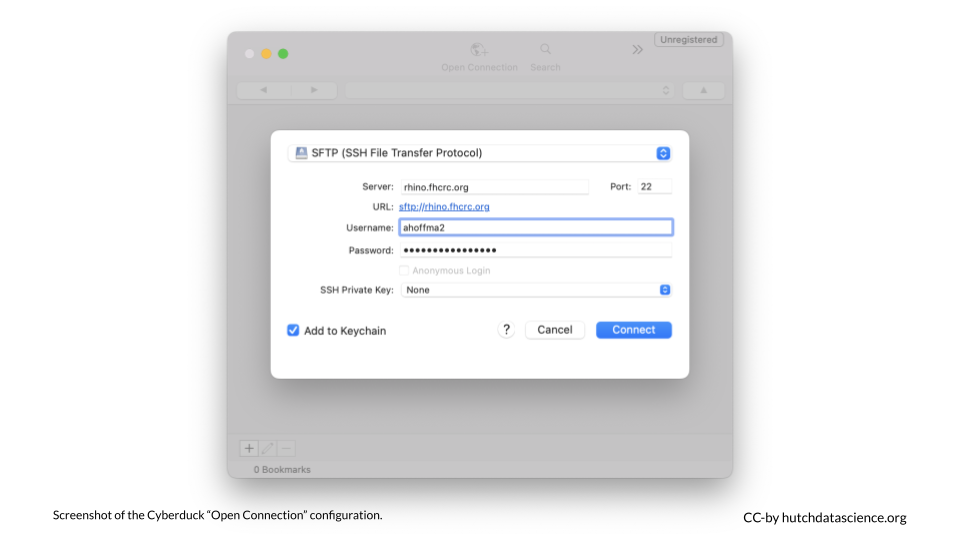
\includegraphics[width=1\linewidth]{resources/images/01-101_files/figure-latex//1BQxrVYdKZTbpCaF-i_q9w7s9x034lEXpQZDU-Sl09cs_g1579ffd7b01_12_28}

Click ``Allow''. You can also check the box to indicate ``Always''.

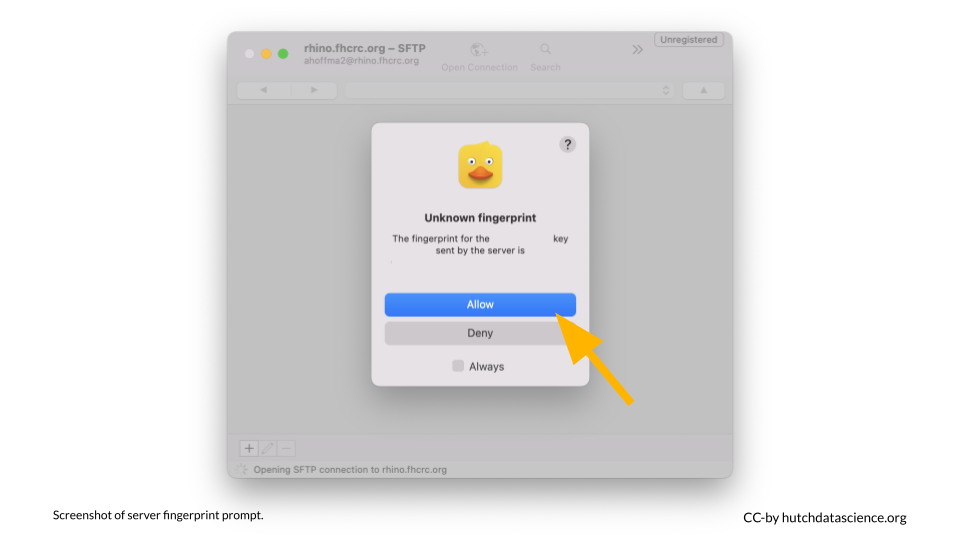
\includegraphics[width=1\linewidth]{resources/images/01-101_files/figure-latex//1BQxrVYdKZTbpCaF-i_q9w7s9x034lEXpQZDU-Sl09cs_g1579ffd7b01_12_33}

You should see your script file ``\texttt{01.sh}'' and the log file.

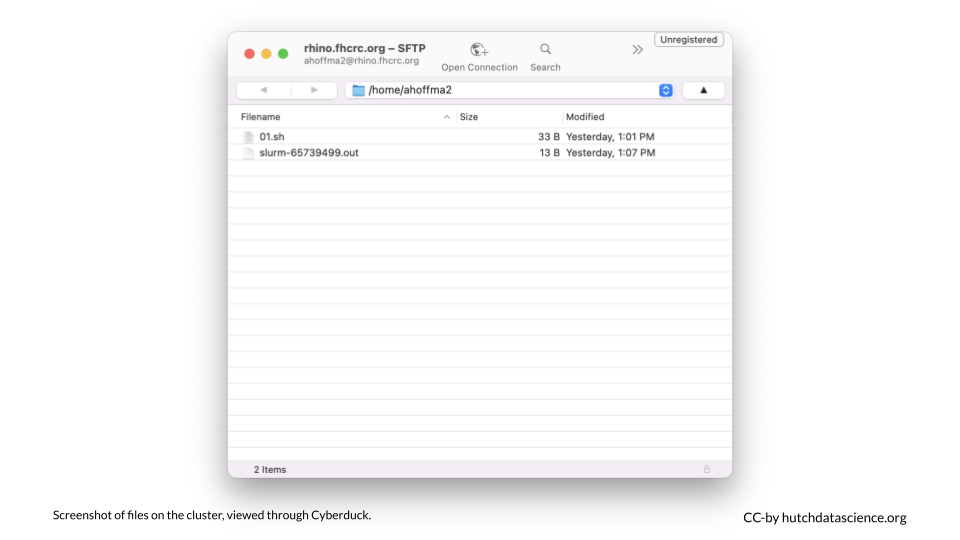
\includegraphics[width=1\linewidth]{resources/images/01-101_files/figure-latex//1BQxrVYdKZTbpCaF-i_q9w7s9x034lEXpQZDU-Sl09cs_g1579ffd7b01_12_37}

\hypertarget{download-and-edit-the-script}{%
\section{Download and Edit the Script}\label{download-and-edit-the-script}}

\begin{itemize}
\tightlist
\item
  Right click on ``\texttt{01.sh}'' and select ``Download''
\item
  You will see a ``Transfers'' prompt open, and the \texttt{01.sh} file should now appear in your Downloads folder
\item
  Open the \texttt{01.sh} file
\end{itemize}

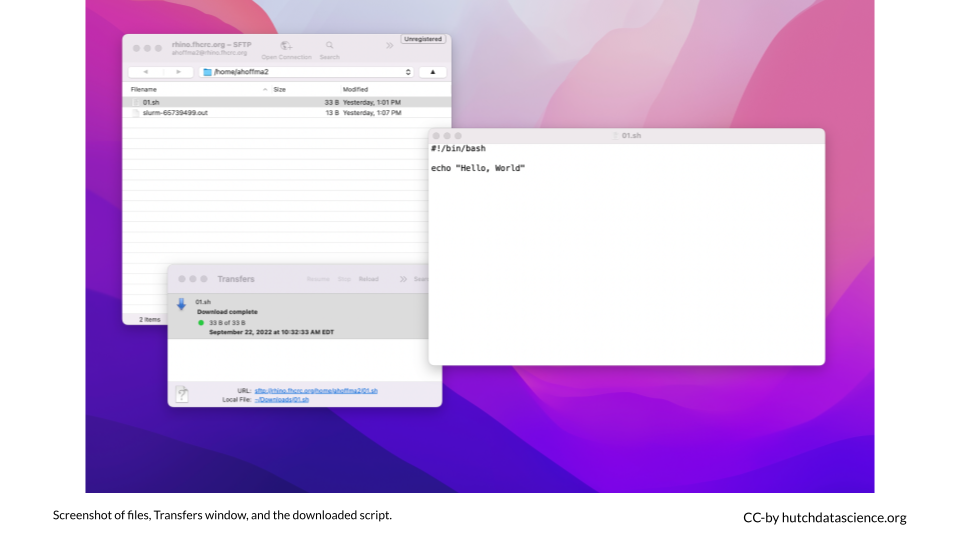
\includegraphics[width=1\linewidth]{resources/images/01-101_files/figure-latex//1BQxrVYdKZTbpCaF-i_q9w7s9x034lEXpQZDU-Sl09cs_g1579ffd7b01_12_41}

Edit the message to include your name and save the file. Rename the file \texttt{01-name.sh}

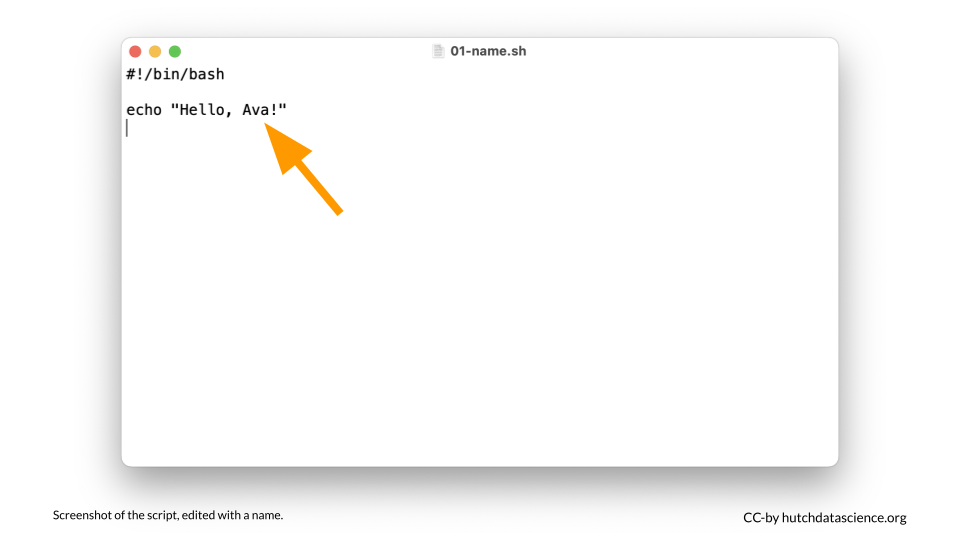
\includegraphics[width=1\linewidth]{resources/images/01-101_files/figure-latex//1BQxrVYdKZTbpCaF-i_q9w7s9x034lEXpQZDU-Sl09cs_g1579ffd7b01_12_45}

\hypertarget{upload-the-new-script}{%
\section{Upload the New Script}\label{upload-the-new-script}}

From your Downloads folder, simply drag the file to Cyberduck.

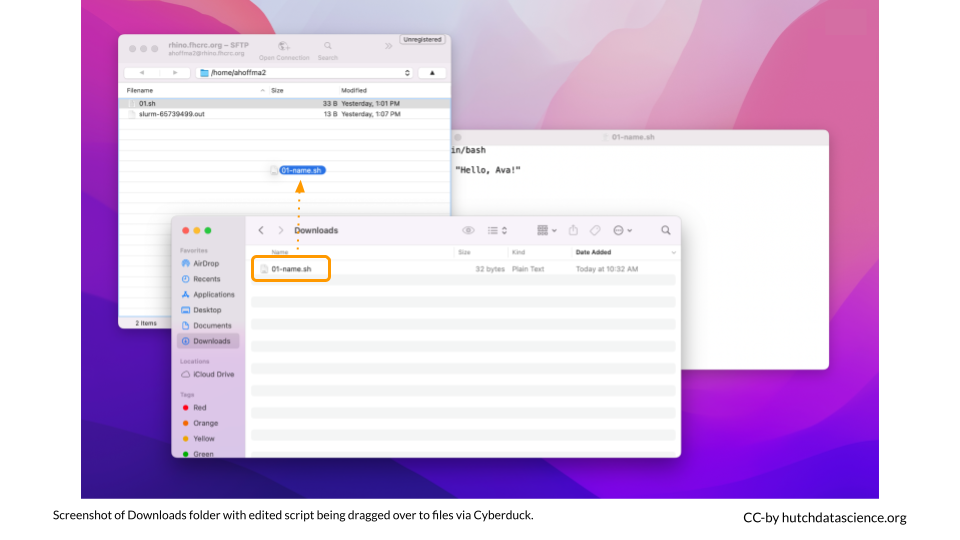
\includegraphics[width=1\linewidth]{resources/images/01-101_files/figure-latex//1BQxrVYdKZTbpCaF-i_q9w7s9x034lEXpQZDU-Sl09cs_g1579ffd7b01_12_49}

You should now see the new script among your cluster files.

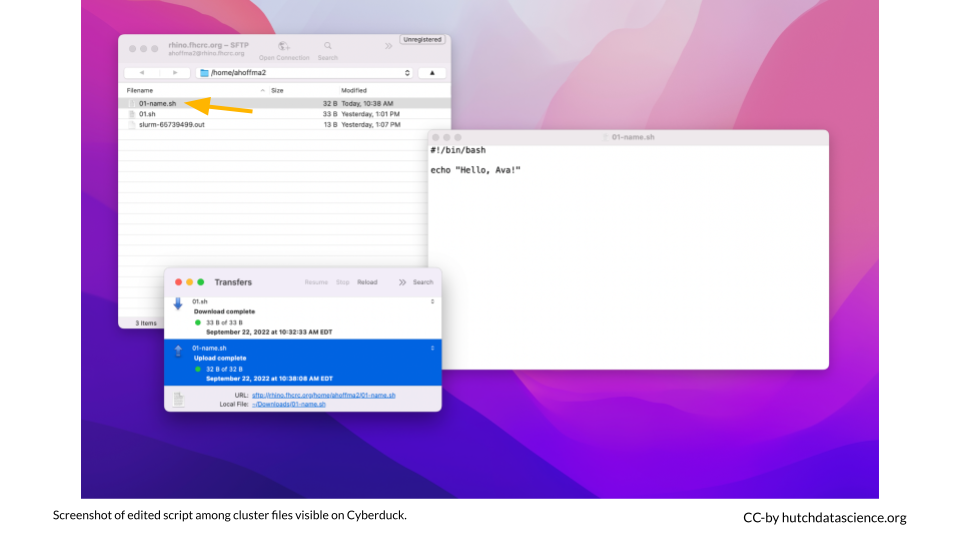
\includegraphics[width=1\linewidth]{resources/images/01-101_files/figure-latex//1BQxrVYdKZTbpCaF-i_q9w7s9x034lEXpQZDU-Sl09cs_g15cf3fa00a4_0_6}

\hypertarget{run-the-new-script}{%
\section{Run the New Script}\label{run-the-new-script}}

Return to your Terminal. Submit a job with your new script by running the following. When you type \texttt{ls} you should see a new log file!

\begin{verbatim}
sbatch 01-name.sh
\end{verbatim}

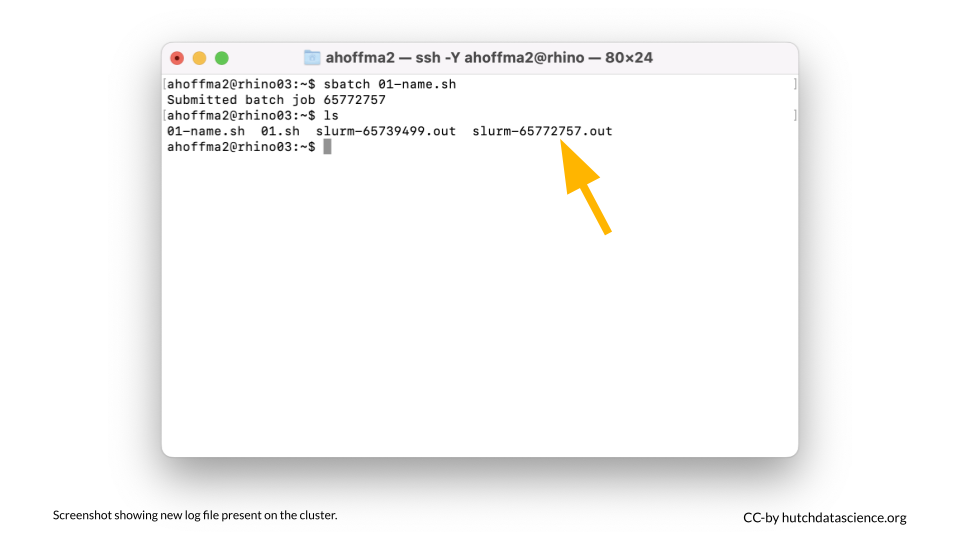
\includegraphics[width=1\linewidth]{resources/images/01-101_files/figure-latex//1BQxrVYdKZTbpCaF-i_q9w7s9x034lEXpQZDU-Sl09cs_gff2211b72f_1_0}

The job numbers included in log file names generally increase in number. The greater the number, the more recently the job was run.

Use the \texttt{cat} command to inspect the log. The message should show the new text that you added!

\begin{verbatim}
cat slurm-<your-number-here>.out
\end{verbatim}

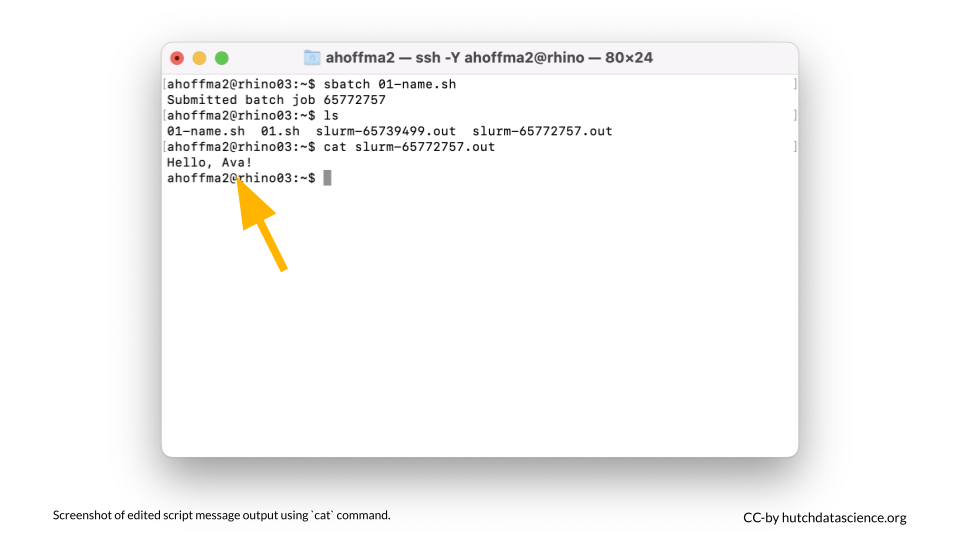
\includegraphics[width=1\linewidth]{resources/images/01-101_files/figure-latex//1BQxrVYdKZTbpCaF-i_q9w7s9x034lEXpQZDU-Sl09cs_gff2211b72f_1_6}

\hypertarget{interactive-session}{%
\chapter{Interactive Session}\label{interactive-session}}

While using the cluster, you might need to build and test jobs interactively before running them. Luckily, you can launch an interactive session, or node. Interactive nodes are dedicated computing resources that are meant to be used interactively, rather than through a job submission system. Interactive nodes are also useful if you have to install specific software.

\hypertarget{starting-the-session}{%
\section{Starting the Session}\label{starting-the-session}}

Start an interactive node by running the command:

\begin{verbatim}
grabnode
\end{verbatim}

You will be prompted with several questions about the type of interactive node you want. We don't need anything fancy, so we will set up the node to use minimal resources. You can enter the following:

\begin{itemize}
\tightlist
\item
  \emph{How many CPUs/cores would you like to grab on the node?} \textbf{1}
\item
  \emph{How much memory (GB) would you like to grab?} \textbf{20}
\item
  \emph{Please enter the max number of days you would like to grab this node:} \textbf{1}
\item
  \emph{Do you need a GPU?} \textbf{N}
\item
  When prompted, enter your password
\end{itemize}

The CPU, or Central Processing Unit, is the brain of the computer that performs and orchestrates computational tasks. Modern computers often perform multiple tasks at once, ranging from 4 tasks on a typical laptop to 48 tasks or more on higher end servers.

RAM, or Random Access Memory, is often simply referred to as memory. This short term memory holds the information that the CPU needs to perform calculations. One distinctive feature of memory is that it is short term. In other words, when the electricity is shut off, the data stored in memory disappears. To save the CPU's work, you usually save files to your computer. Running highly complicated analyses or algorithms can often require additional memory resources.

The \href{https://www.intel.com/content/www/us/en/products/docs/processors/what-is-a-gpu.html}{GPU}, or Graphics Processing Unit, is similar to the CPU. The GPU was originally designed to quickly render graphics (such as for video games), but today can be used to run complex artificial intelligence applications or computationally intensive jobs.

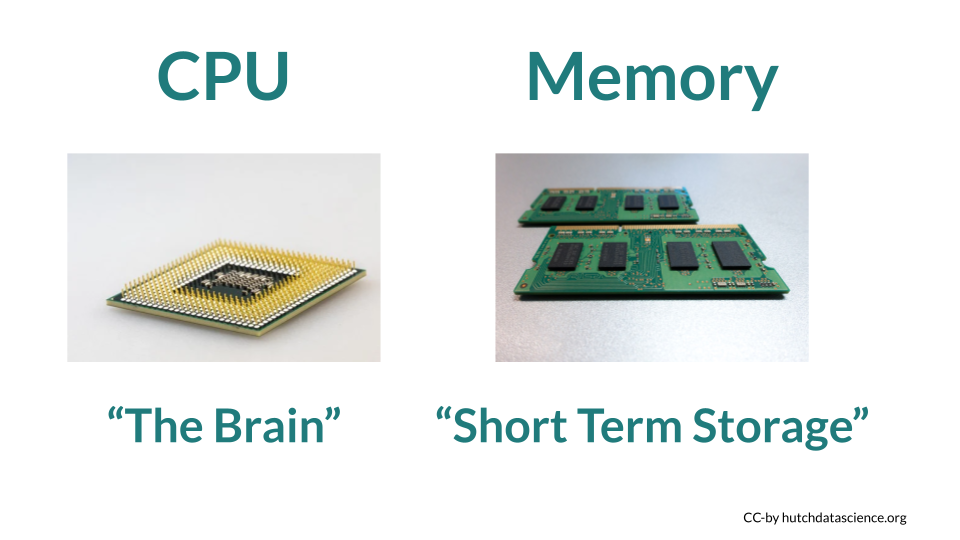
\includegraphics[width=1\linewidth]{resources/images/01-101_files/figure-latex//1BQxrVYdKZTbpCaF-i_q9w7s9x034lEXpQZDU-Sl09cs_gff2211b72f_1_26}

You will see that you are now logged on to a ``gizmo'' node instead of a ``rhino'' node.

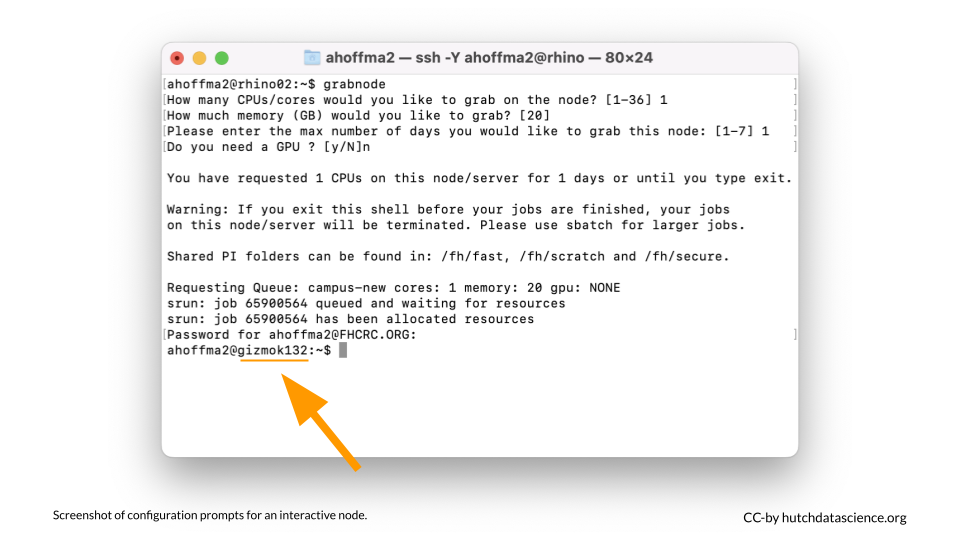
\includegraphics[width=1\linewidth]{resources/images/01-101_files/figure-latex//1BQxrVYdKZTbpCaF-i_q9w7s9x034lEXpQZDU-Sl09cs_gff2211b72f_1_50}

\hypertarget{running-interactive-commands}{%
\section{Running Interactive Commands}\label{running-interactive-commands}}

You can start the session by running a similar command as we used in the job we submitted via script. Echo a message by running:

\begin{verbatim}
echo "Hello, again!"
\end{verbatim}

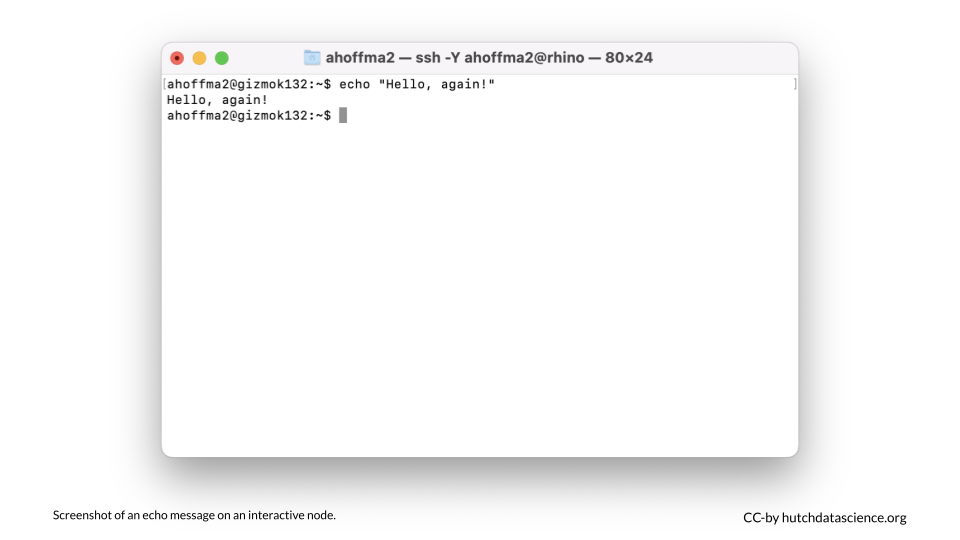
\includegraphics[width=1\linewidth]{resources/images/01-101_files/figure-latex//1BQxrVYdKZTbpCaF-i_q9w7s9x034lEXpQZDU-Sl09cs_gff2211b72f_1_58}

Let's get a bit more advanced. We can load a preconfigured software bundle called a module. This is very convenient because it means we don't need to install anything manually! In this example, we will load a module containing \href{https://www.r-project.org/}{R} version 4.2.0.

\begin{verbatim}
ml R/4.2.0-foss-2021b
\end{verbatim}

Next, launch R:

\begin{verbatim}
R
\end{verbatim}

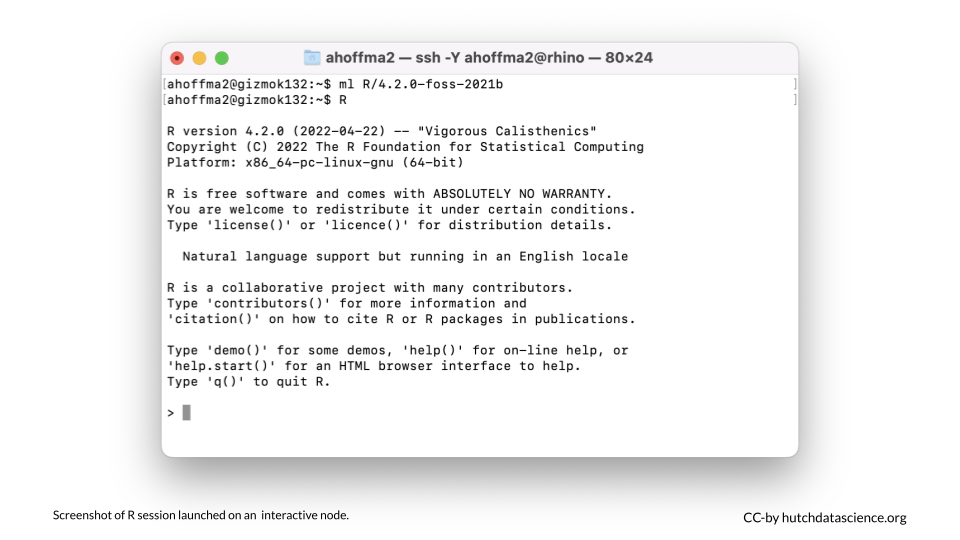
\includegraphics[width=1\linewidth]{resources/images/01-101_files/figure-latex//1BQxrVYdKZTbpCaF-i_q9w7s9x034lEXpQZDU-Sl09cs_gff2211b72f_1_65}

You can play around with R here. For example, you might run:

\begin{verbatim}
head(mtcars)
\end{verbatim}

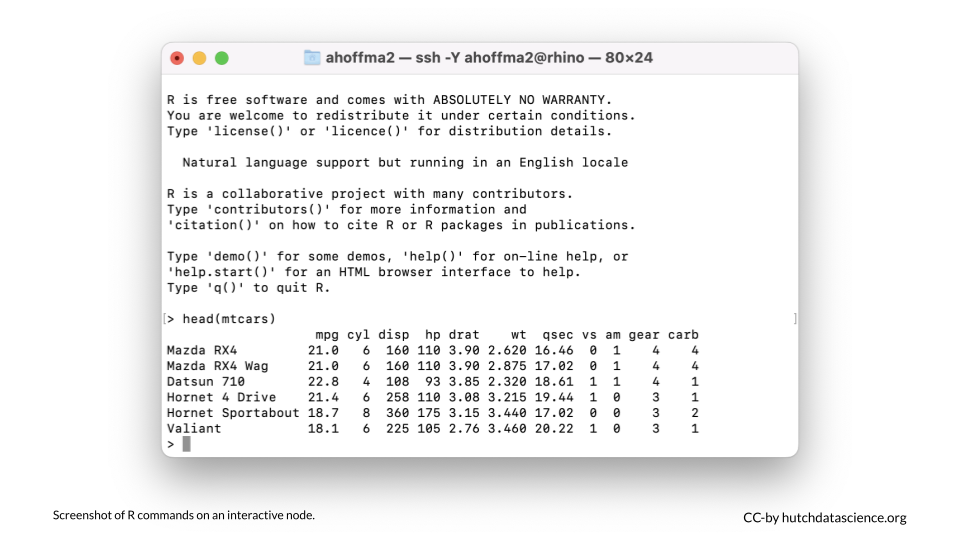
\includegraphics[width=1\linewidth]{resources/images/01-101_files/figure-latex//1BQxrVYdKZTbpCaF-i_q9w7s9x034lEXpQZDU-Sl09cs_gff2211b72f_1_72}

Close the R session by typing:

\begin{verbatim}
q()
\end{verbatim}

Close the interactive node by typing:

\begin{verbatim}
exit
\end{verbatim}

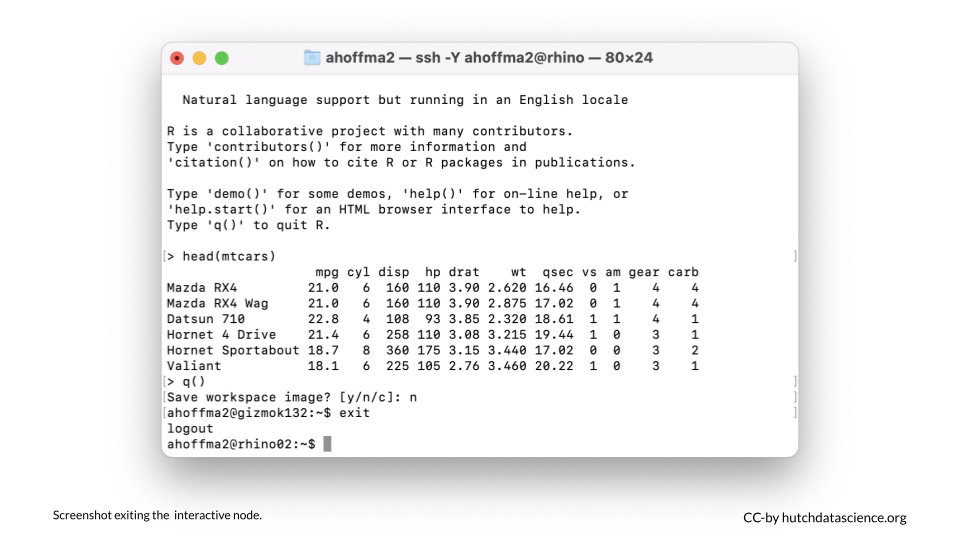
\includegraphics[width=1\linewidth]{resources/images/01-101_files/figure-latex//1BQxrVYdKZTbpCaF-i_q9w7s9x034lEXpQZDU-Sl09cs_gff2211b72f_1_82}

\texttt{grabnode}

This command starts an interactive session, or node.

\textbf{CPU}

A computer component that performs and orchestrates computational tasks.

\textbf{Memory}

A computer component that stores calculations and information in the short term.

\hypertarget{part-assessment}{%
\part*{Assessment}\label{part-assessment}}
\addcontentsline{toc}{part}{Assessment}

\hypertarget{cluster-101-self-test}{%
\chapter{Cluster 101 Self Test}\label{cluster-101-self-test}}

\hypertarget{part-appendix}{%
\part*{Appendix}\label{part-appendix}}
\addcontentsline{toc}{part}{Appendix}

\hypertarget{help}{%
\chapter{Where to get help}\label{help}}

We want to help! Here are some ways you can get help for your work on the cluster.

\hypertarget{submit-a-ticket}{%
\section*{Submit a Ticket}\label{submit-a-ticket}}
\addcontentsline{toc}{section}{Submit a Ticket}

Submitting a good ticket helps the SciComp Team address your needs quickly and efficiently. We suggest you submit the following in a ticket:

\begin{enumerate}
\def\labelenumi{\arabic{enumi}.}
\tightlist
\item
\item
\item
\end{enumerate}

\hypertarget{visit-the-sciwiki}{%
\section*{Visit the SciWiki}\label{visit-the-sciwiki}}
\addcontentsline{toc}{section}{Visit the SciWiki}

The SciWiki \href{https://sciwiki.fredhutch.org/scicomputing/comp_index/}{Scientific Computing page} is full of useful tips and guides.

\hypertarget{feedback}{%
\chapter{Provide Feedback}\label{feedback}}

Please submit an issue at our \href{https://github.com/fhdsl/FH_Cluster_Guide/issues/new}{GitHub repository}. You can also click the edit button on the top of the page in question.

\hypertarget{faq-troubleshooting}{%
\chapter{FAQ / Troubleshooting}\label{faq-troubleshooting}}

\hypertarget{faq}{%
\section{FAQ}\label{faq}}

Here are some questions you might have.

\hypertarget{manual-putty}{%
\subsection{How can I manually install PuTTY?}\label{manual-putty}}

Click to view steps

\begin{enumerate}
\def\labelenumi{\arabic{enumi}.}
\item
  Click \href{https://www.chiark.greenend.org.uk/~sgtatham/putty/latest.html}{here} to install the latest version of PuTTY. You will choose the 64-bit x86 installation with few exceptions.

  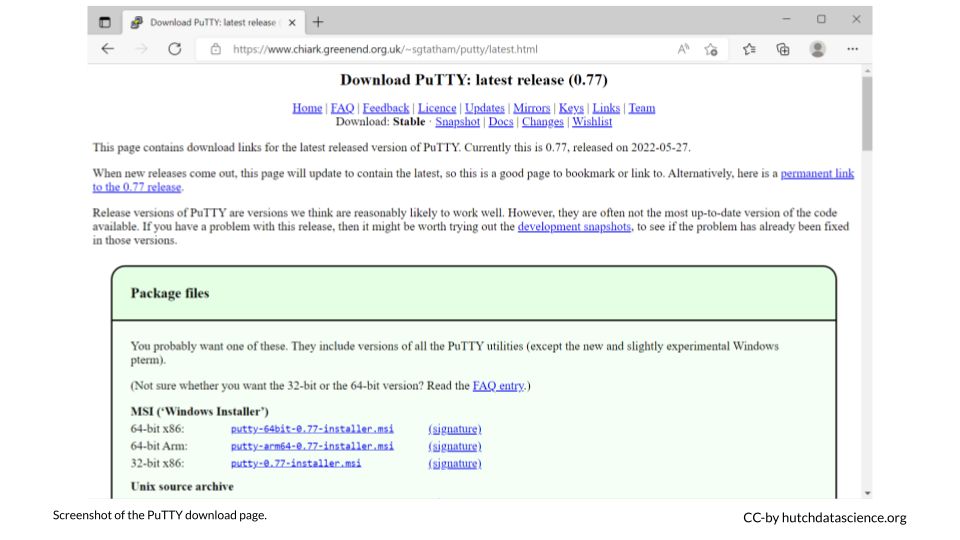
\includegraphics[width=1\linewidth]{faq_files/figure-latex//1BQxrVYdKZTbpCaF-i_q9w7s9x034lEXpQZDU-Sl09cs_g15643d101eb_4_6}
\item
  Click through to install via the Setup Wizard.
\end{enumerate}

\hypertarget{troubleshooting}{%
\section{Troubleshooting}\label{troubleshooting}}

Here are some issues you might encounter.

\hypertarget{ssh-could-not-resolve-hostname-rhino-nodename-nor-servname-provided-or-not-known}{%
\subsection*{\texorpdfstring{\texttt{ssh:\ Could\ not\ resolve\ hostname\ rhino:\ nodename\ nor\ servname\ provided,\ or\ not\ known}}{ssh: Could not resolve hostname rhino: nodename nor servname provided, or not known}}\label{ssh-could-not-resolve-hostname-rhino-nodename-nor-servname-provided-or-not-known}}
\addcontentsline{toc}{subsection}{\texttt{ssh:\ Could\ not\ resolve\ hostname\ rhino:\ nodename\ nor\ servname\ provided,\ or\ not\ known}}

Click to view steps

This error means that your computer is having trouble connecting to rhino. Ensure one of the following is true:

\begin{enumerate}
\def\labelenumi{\arabic{enumi}.}
\tightlist
\item
  You are connected to the Fred Hutch wifi network on campus.
\item
  You are connected to the Fred Hutch VPN
\item
  You are plugged into an ethernet cable on campus that taps into the Fred Hutch network. Note that not all ethernet wall jacks have this capability, so try another jack if you are having trouble. Please email the IT helpdesk and include your office number and the number on the jack if you find a jack that isn't working.
\end{enumerate}

\hypertarget{ssh-connect-to-host-rhino-port-22-undefined-error-0}{%
\subsection*{\texorpdfstring{\texttt{ssh:\ connect\ to\ host\ rhino\ port\ 22:\ Undefined\ error:\ 0}}{ssh: connect to host rhino port 22: Undefined error: 0}}\label{ssh-connect-to-host-rhino-port-22-undefined-error-0}}
\addcontentsline{toc}{subsection}{\texttt{ssh:\ connect\ to\ host\ rhino\ port\ 22:\ Undefined\ error:\ 0}}

Click to view steps

This likely indicates a disruption to your internet connection and/or VPN. Ensure you are connected to the internet and connected to the Fred Hutch network on campus or the VPN.

\hypertarget{connection-failed-message-in-cyberduck}{%
\subsection*{\texorpdfstring{\texttt{Connection\ failed} message in Cyberduck}{Connection failed message in Cyberduck}}\label{connection-failed-message-in-cyberduck}}
\addcontentsline{toc}{subsection}{\texttt{Connection\ failed} message in Cyberduck}

Click to view steps

This likely indicates a disruption to your internet connection and/or VPN. Ensure you are connected to the internet and connected to the Fred Hutch network on campus or the VPN.

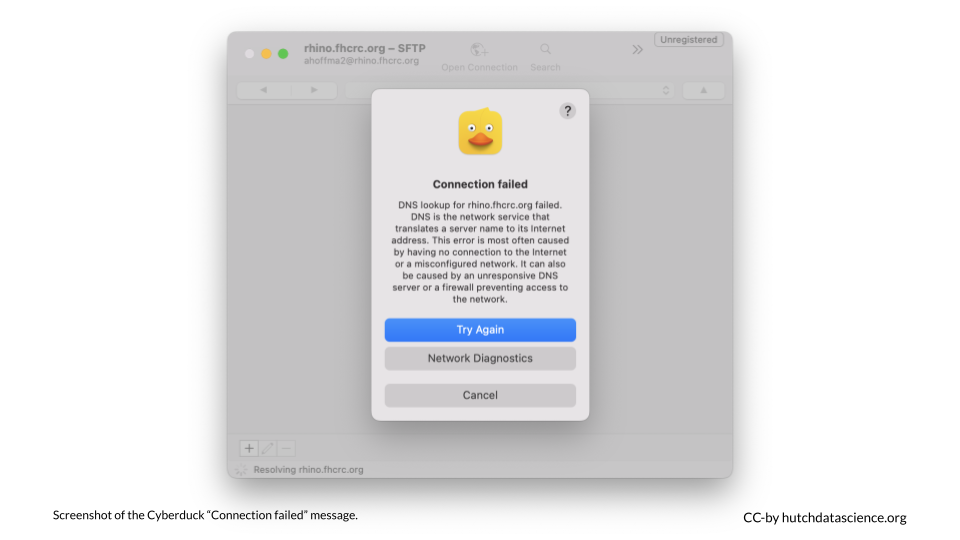
\includegraphics[width=1\linewidth]{faq_files/figure-latex//1BQxrVYdKZTbpCaF-i_q9w7s9x034lEXpQZDU-Sl09cs_gff2211b72f_1_16}

\hypertarget{about-the-authors}{%
\chapter*{About the Authors}\label{about-the-authors}}
\addcontentsline{toc}{chapter}{About the Authors}

These credits are based on our \href{https://github.com/jhudsl/OTTR_Template/wiki/How-to-give-credits}{course contributors table guidelines}.

~
~

\begin{longtable}[]{@{}
  >{\raggedright\arraybackslash}p{(\columnwidth - 2\tabcolsep) * \real{0.58}}
  >{\raggedright\arraybackslash}p{(\columnwidth - 2\tabcolsep) * \real{0.42}}@{}}
\toprule
\begin{minipage}[b]{\linewidth}\raggedright
Credits
\end{minipage} & \begin{minipage}[b]{\linewidth}\raggedright
Names
\end{minipage} \\
\midrule
\endhead
\textbf{Pedagogy} & \\
Lead Content Instructor(s) & \href{link\%20to\%20personal\%20website}{FirstName LastName} \\
Lecturer(s) (include chapter name/link in parentheses if only for specific chapters) - make new line if more than one chapter involved & Delivered the course in some way - video or audio \\
Content Author(s) (include chapter name/link in parentheses if only for specific chapters) - make new line if more than one chapter involved & If any other authors besides lead instructor \\
Content Contributor(s) (include section name/link in parentheses) - make new line if more than one section involved & Wrote less than a chapter \\
Content Editor(s)/Reviewer(s) & Checked your content \\
Content Director(s) & Helped guide the content direction \\
Content Consultants (include chapter name/link in parentheses or word ``General'') - make new line if more than one chapter involved & Gave high level advice on content \\
Acknowledgments & Gave small assistance to content but not to the level of consulting \\
\textbf{Production} & \\
Content Publisher(s) & Helped with publishing platform \\
Content Publishing Reviewer(s) & Reviewed overall content and aesthetics on publishing platform \\
\textbf{Technical} & \\
Course Publishing Engineer(s) & Helped with the code for the technical aspects related to the specific course generation \\
Template Publishing Engineers & \href{https://www.cansavvy.com/}{Candace Savonen}, \href{https://carriewright11.github.io/}{Carrie Wright} \\
Publishing Maintenance Engineer & \href{https://www.cansavvy.com/}{Candace Savonen} \\
Technical Publishing Stylists & \href{https://carriewright11.github.io/}{Carrie Wright}, \href{https://www.cansavvy.com/}{Candace Savonen} \\
Package Developers (\href{https://github.com/jhudsl/ottrpal}{ottrpal}) \href{https://www.cansavvy.com/}{Candace Savonen}, \href{https://johnmuschelli.com/}{John Muschelli}, \href{https://carriewright11.github.io/}{Carrie Wright} & \\
\textbf{Art and Design} & \\
Illustrator(s) & Created graphics for the course \\
Figure Artist(s) & Created figures/plots for course \\
Videographer(s) & Filmed videos \\
Videography Editor(s) & Edited film \\
Audiographer(s) & Recorded audio \\
Audiography Editor(s) & Edited audio recordings \\
\textbf{Funding} & \\
Funder(s) & Institution/individual who funded course including grant number \\
Funding Staff & Staff members who help with funding \\
\bottomrule
\end{longtable}

~

\begin{verbatim}
## - Session info ---------------------------------------------------------------
##  setting  value                       
##  version  R version 4.0.2 (2020-06-22)
##  os       Ubuntu 20.04.3 LTS          
##  system   x86_64, linux-gnu           
##  ui       X11                         
##  language (EN)                        
##  collate  en_US.UTF-8                 
##  ctype    en_US.UTF-8                 
##  tz       Etc/UTC                     
##  date     2022-09-23                  
## 
## - Packages -------------------------------------------------------------------
##  package     * version    date       lib source                            
##  assertthat    0.2.1      2019-03-21 [1] RSPM (R 4.0.3)                    
##  bookdown      0.24       2022-02-15 [1] Github (rstudio/bookdown@88bc4ea) 
##  callr         3.4.4      2020-09-07 [1] RSPM (R 4.0.2)                    
##  cli           2.0.2      2020-02-28 [1] RSPM (R 4.0.0)                    
##  crayon        1.3.4      2017-09-16 [1] RSPM (R 4.0.0)                    
##  desc          1.2.0      2018-05-01 [1] RSPM (R 4.0.3)                    
##  devtools      2.3.2      2020-09-18 [1] RSPM (R 4.0.3)                    
##  digest        0.6.25     2020-02-23 [1] RSPM (R 4.0.0)                    
##  ellipsis      0.3.1      2020-05-15 [1] RSPM (R 4.0.3)                    
##  evaluate      0.14       2019-05-28 [1] RSPM (R 4.0.3)                    
##  fansi         0.4.1      2020-01-08 [1] RSPM (R 4.0.0)                    
##  fs            1.5.0      2020-07-31 [1] RSPM (R 4.0.3)                    
##  glue          1.6.1      2022-01-22 [1] CRAN (R 4.0.2)                    
##  htmltools     0.5.0      2020-06-16 [1] RSPM (R 4.0.1)                    
##  knitr         1.33       2022-02-15 [1] Github (yihui/knitr@a1052d1)      
##  lifecycle     1.0.0      2021-02-15 [1] CRAN (R 4.0.2)                    
##  magrittr      2.0.2      2022-01-26 [1] CRAN (R 4.0.2)                    
##  memoise       1.1.0      2017-04-21 [1] RSPM (R 4.0.0)                    
##  pkgbuild      1.1.0      2020-07-13 [1] RSPM (R 4.0.2)                    
##  pkgload       1.1.0      2020-05-29 [1] RSPM (R 4.0.3)                    
##  prettyunits   1.1.1      2020-01-24 [1] RSPM (R 4.0.3)                    
##  processx      3.4.4      2020-09-03 [1] RSPM (R 4.0.2)                    
##  ps            1.3.4      2020-08-11 [1] RSPM (R 4.0.2)                    
##  purrr         0.3.4      2020-04-17 [1] RSPM (R 4.0.3)                    
##  R6            2.4.1      2019-11-12 [1] RSPM (R 4.0.0)                    
##  remotes       2.2.0      2020-07-21 [1] RSPM (R 4.0.3)                    
##  rlang         0.4.10     2022-02-15 [1] Github (r-lib/rlang@f0c9be5)      
##  rmarkdown     2.10       2022-02-15 [1] Github (rstudio/rmarkdown@02d3c25)
##  rprojroot     2.0.2      2020-11-15 [1] CRAN (R 4.0.2)                    
##  sessioninfo   1.1.1      2018-11-05 [1] RSPM (R 4.0.3)                    
##  stringi       1.5.3      2020-09-09 [1] RSPM (R 4.0.3)                    
##  stringr       1.4.0      2019-02-10 [1] RSPM (R 4.0.3)                    
##  testthat      3.0.1      2022-02-15 [1] Github (R-lib/testthat@e99155a)   
##  usethis       2.1.5.9000 2022-02-15 [1] Github (r-lib/usethis@57b109a)    
##  withr         2.3.0      2020-09-22 [1] RSPM (R 4.0.2)                    
##  xfun          0.32       2022-08-10 [1] CRAN (R 4.0.2)                    
##  yaml          2.2.1      2020-02-01 [1] RSPM (R 4.0.3)                    
## 
## [1] /usr/local/lib/R/site-library
## [2] /usr/local/lib/R/library
\end{verbatim}

\hypertarget{references}{%
\chapter*{References}\label{references}}
\addcontentsline{toc}{chapter}{References}

\end{document}
